\documentclass[11pt,a4paper]{article}
\usepackage[T1]{fontenc}
\usepackage[utf8]{inputenc}
\usepackage{lmodern,microtype}
\usepackage[top=2.35cm,bottom=2.25cm,left=2.25cm,right=2.25cm]{geometry}
\usepackage{amsmath,booktabs,tabularx,array,graphicx,xcolor,caption,fancyhdr}
\usepackage{hyperref}
\definecolor{navy}{HTML}{14283E}
\definecolor{teal}{HTML}{116A6B}
\definecolor{muted}{HTML}{516475}
\hypersetup{colorlinks=true,linkcolor=teal,citecolor=teal,urlcolor=teal,
  pdftitle={Incremental Structure from Motion on Two NTU Campus Sculptures},
  pdfsubject={AI6121 Computer Vision Group Project}}
\setlength{\headheight}{15pt}
\pagestyle{fancy}
\fancyhf{}
\fancyhead[L]{\small\color{muted}AI6121 Computer Vision}
\fancyhead[R]{\small\color{muted}Structure from Motion}
\fancyfoot[R]{\small\color{muted}\thepage}
\renewcommand{\headrulewidth}{0.35pt}
\setlength{\parindent}{0pt}
\setlength{\parskip}{0.58em}
\captionsetup{font=small,labelfont=bf,skip=5pt,hypcap=false}
\renewcommand{\arraystretch}{1.19}
\newcolumntype{Y}{>{\raggedright\arraybackslash}X}
\newcolumntype{C}{>{\centering\arraybackslash}X}
\newcommand{\code}[1]{\texttt{\detokenize{#1}}}
\newcommand{\surfacecomparison}[1]{%
  {\small\begin{tabularx}{\linewidth}{@{}CCC@{}}
  \textbf{Colored surface} & \textbf{Wireframe} & \textbf{Face normals}
  \end{tabularx}}\par\vspace{4pt}%
  \includegraphics[width=\linewidth,trim=0 44bp 0 63bp,clip]{#1}}
\graphicspath{{../outputs/final/fern/figures/}{../outputs/final/red-solace/figures/}%
  {../outputs/final/fern/surface/}{../outputs/final/red-solace/surface/}%
  {../outputs/case-study/}}

\begin{document}
\begin{titlepage}
\thispagestyle{empty}
\raggedright
\vspace*{1.5cm}
{\large\bfseries\color{teal} NANYANG TECHNOLOGICAL UNIVERSITY\par}
\vspace{0.35cm}
{\large AI6121 Computer Vision \quad | \quad Group Project Report\par}
\vspace{1.2cm}
{\fontsize{34}{39}\selectfont\bfseries\color{navy}
Incremental Structure\\from Motion on Two\\NTU Campus Sculptures\par}
\vspace{0.5cm}
{\Large\color{muted} Fern and Red Solace\par}
\vspace{1.1cm}
{\large\bfseries Group members\par}
\vspace{0.2cm}
\begin{tabularx}{0.91\linewidth}{@{}lYY@{}}
\toprule
 & \textbf{Full name} & \textbf{Matriculation number}\\
\midrule
1 & [Enter full name] & [Enter matriculation number]\\
2 & [Enter full name] & [Enter matriculation number]\\
3 & [Enter full name] & [Enter matriculation number]\\
4 & [Enter full name] & [Enter matriculation number]\\
5 & [Enter full name] & [Enter matriculation number]\\
\bottomrule
\end{tabularx}
\vspace{0.3cm}

{\small\color{muted} Complete the member details and remove unused rows before submission.\par}
\vfill
{\large\bfseries\color{navy} Generative AI usage declaration\par}
{\small The original project draft records assistance from Google Gemini and
DeepMind Antigravity with matching prototypes, debugging and the initial
report. OpenAI Codex assisted with reviewing and revising the implementation,
running and analysing experiments, and revising this report.\par}
\vspace{0.55cm}
{\small\color{muted} November 2026 \quad | \quad Academic Year 2026/2027\par}
\end{titlepage}

\section*{Abstract}
This project reconstructs two NTU campus sculptures using incremental
Structure from Motion (SfM) followed by image-based surface reconstruction.
The revised SfM pipeline selects keyframes by overlap, motion and sharpness,
tests multiple initial pairs and builds consistent tracks across views. Bundle
adjustment refines camera poses, points and a shared focal parameter per clip.
Rectified stereo then estimates pixel-level depth using the recovered cameras.

On the same 50 archived Fern frames with fixed feature matches, the original
and revised pipelines register 6 and 26 frames, respectively. The revised
single-clip experiments register 24 of 72 Fern frames and all 40 Red Solace
frames. Localizing additional frames in the Red Solace reference map gives
73 registered poses across six clips. Red Solace supports a surface with
63,770 triangles fused from 35 reference depth maps. Fern's single clip
retains a gap in its camera trajectory. A separate run using archived clips 002 and 004 yields
22,557 triangles over the visible wooden ribs and part of the base. The report
compares colored surfaces, wireframes and face normals, and relates the
remaining gaps to view coverage.

\section{Task and data}
Given overlapping views of a static scene, SfM estimates camera poses and 3D
structure jointly \cite{hartley,schonberger}. We reconstruct the curved wooden
Fern sculpture and the mosaic-covered Red Solace sculpture. Fern presents
repeated slats and large changes in framing. The mosaic provides more distinct
local texture, although shadows and occlusions still affect correspondences.

\begin{center}
\small
\begin{tabularx}{\linewidth}{@{}lrrYr@{}}
\toprule
\textbf{Scene} & \textbf{Photos} & \textbf{Clips} & \textbf{Revised video input} & \textbf{Keyframes}\\
\midrule
Fern & 74 & 8 & \code{Fern/video/006.mp4} & 72\\
Red Solace & 41 & 6 & \code{Red_Solace/video/003.mp4} & 40\\
\bottomrule
\end{tabularx}
\end{center}

The original dataset contains 115 photos and 14 clips. The revised benchmark
uses one continuous clip per sculpture. The archived 50-frame Fern replay is a
separate controlled experiment using frames from clips 002 and 004. Photos
remain supported by the loader. The revised benchmark evaluates video inputs.

\section{Revised pipeline}
\subsection{Continuous video and adaptive keyframes}
The sampler divides each clip into temporal windows and evaluates candidate
frames with forward-backward Lucas-Kanade tracking. It favours a large fraction
of consistently tracked corners, moderate median image displacement and high
Laplacian-variance sharpness. It skips near duplicates and can retain a
weak-overlap candidate to cover a time interval. Image displacement guides
sampling. Geometric parallax is checked later. Original frame indices and
timestamps are recorded for auditing.

\clearpage
\subsection{Verified matches, initialization and incremental registration}
The image long edge is limited to 1,280 pixels. The main experiments request
2,400 RootSIFT features per view. RootSIFT applies an elementwise square root to
the L1-normalized SIFT descriptor \cite{rootsift}. The matcher applies a
nearest-neighbour ratio of 0.78 and a mutual nearest-neighbour check. SIFT uses
L2 distance, while ORB preserves its binary representation and uses Hamming
distance. Fern uses local temporal pairs and sampled loop candidates. Red
Solace uses exhaustive pairing.

\textbf{Two-view verification.} The mapper robustly estimates a fundamental
matrix and a homography. It retains an image-pair edge when a model supplies
sufficient inliers. Adjacent frames can contribute feature tracks even when
their baseline is too short for initialization. The mapper excludes
homography-dominated seed pairs, estimates the essential matrix on normalized
correspondences, and checks positive depth, triangulation angle and image coverage.

\textbf{Multiple seed probes.} Usable tracks, parallax, image coverage and
support from other views determine the seed ranking. Up to four candidates
are probed, with preference for different time intervals of a single clip.
The strongest probes can grow further. Registered views take precedence
over multi-view track support in selecting the reconstruction.

\textbf{Tracks and pose estimation.} Verified pairs are linked into tracks.
A merge is rejected if it assigns two keypoints from the same image to one
track. Given an existing 3D landmark and a new observation of its track,
EPnP with RANSAC estimates the new pose \cite{epnp}. The mapper refines the
pose on inliers and checks positive depth and spatial spread. It triangulates
new landmarks and rechecks their observations. When growth stalls, a
successful refinement permits another registration attempt.

\subsection{Camera intrinsics and bundle adjustment}
For the uncalibrated video runs, the initial focal length in resized-image
pixels is \(0.95\max(w,h)\), with principal point \((w/2,h/2)\). A JSON calibration
can supply a measured \(K\) and distortion for each source. The loader scales
\(K\) to the working resolution, undistorts the image before feature
extraction, and holds measured intrinsics fixed. The reported video runs use
the focal prior because measured calibration was unavailable.

A camera projects \(X_j\) to \(\pi(K_i(R_iX_j+t_i))\), where \(\pi\) divides by
the third homogeneous coordinate. Sparse bundle adjustment \cite{triggs}
minimizes robust reprojection residuals and regularizes the shared focal
scale \(s_g\) for each uncalibrated clip:
\[
\min_{\{R_i,t_i,X_j,s_g\}}\ 
\sum_{(i,j)\in\mathcal{O}}
 \rho\!\left(\pi\!\left(K_i(s_g)(R_iX_j+t_i)\right)-u_{ij}\right)
 + \sum_g \rho\!\left(\lambda_g(s_g-1)\right).
\]
Here \(\mathcal{O}\) is the set of accepted observations and \(\rho\) applies
the Huber penalty componentwise. The first pose and one coordinate of the
second translation fix the similarity gauge. After a successful camera
update, the mapper retriangulates points outside the active optimization
subset and checks their observations.

\clearpage
\subsection{Quality gate and feature-based semi-dense fusion}
The runner attempts semi-dense reconstruction when at least eight views and
60\% of the input views are registered, at least 20\% of sparse tracks have
three or more observations, and the 90th percentile of sparse reprojection
error is at most 4 pixels. These thresholds govern the implementation.

The semi-dense stage selects covisible camera pairs, checks matches against
the estimated epipolar geometry and colour, and merges consistent matches
into tracks. It triangulates points from at least three views and checks
positive depth, ray angle and reprojection error. Spatial deduplication
preserves sparse points and avoids adding nearby copies. The result is a
feature-based point cloud. Sparse and semi-dense figures share one coordinate
frame and equal axis units. Video paths are drawn per clip. Section~\ref{sec:surface}
describes the separate pixel-level depth and surface experiments.

\section{Evaluation}
\label{sec:evaluation}
\subsection{Controlled replay on the same Fern input}
Both pipelines received the same 50 archived JPEG frames, RootSIFT features,
482 raw matched image pairs, initial intrinsics, 2.5-pixel geometry threshold,
and minimum support setting of 22. The comparison measures the combined
mapper revision.

\begin{center}
\small
\begin{tabularx}{\linewidth}{@{}Yrrrr@{}}
\toprule
\textbf{Pipeline} & \textbf{Views} & \textbf{Sparse pts.} &
\textbf{Tracks \(\geq 3\)} & \textbf{Mean error}\\
\midrule
Original & 6/50 & 1,694 & 674 (39.8\%) & 0.937 px\\
Revised & 26/50 & 4,931 & 1,285 (26.1\%) & 1.167 px\\
\bottomrule
\end{tabularx}
\end{center}

The revised run registers 20 more frames and yields more tracks with at least
three observations in absolute terms. Their share falls because the number of
two-view points also grows. The mean residual is measured over each run's own
retained views and observations. This test establishes a coverage gain for this
input. Independent geometric accuracy would require a separate measurement.

\subsection{Single-clip reconstruction}
\begin{center}
\small
\begin{tabularx}{\linewidth}{@{}Yrrrrrr@{}}
\toprule
\textbf{Clip} & \textbf{Views} & \textbf{Sparse} & \textbf{Semi-dense} &
\textbf{Tracks \(\geq 3\)} & \textbf{Median} & \textbf{P90}\\
\midrule
Fern 006 & 24/72 & 4,657 & --- & 67.6\% & 0.761 & 1.962\\
Red Solace 003 & 40/40 & 12,693 & 16,481 & 55.6\% & 0.498 & 1.527\\
\bottomrule
\end{tabularx}
\end{center}

Median and P90 are pixel errors on retained sparse observations. The
semi-dense count includes the sparse points. Fern's registered views occur
from 0 to 11.31 seconds and from 59.94 to 69.78 seconds. Its 33.3\%
registration rate falls below the semi-dense gate. Red Solace registers
all selected frames and adds 3,788 points after multi-view checks.

\clearpage
\subsection{Qualitative results}
\begin{minipage}{\linewidth}
\centering
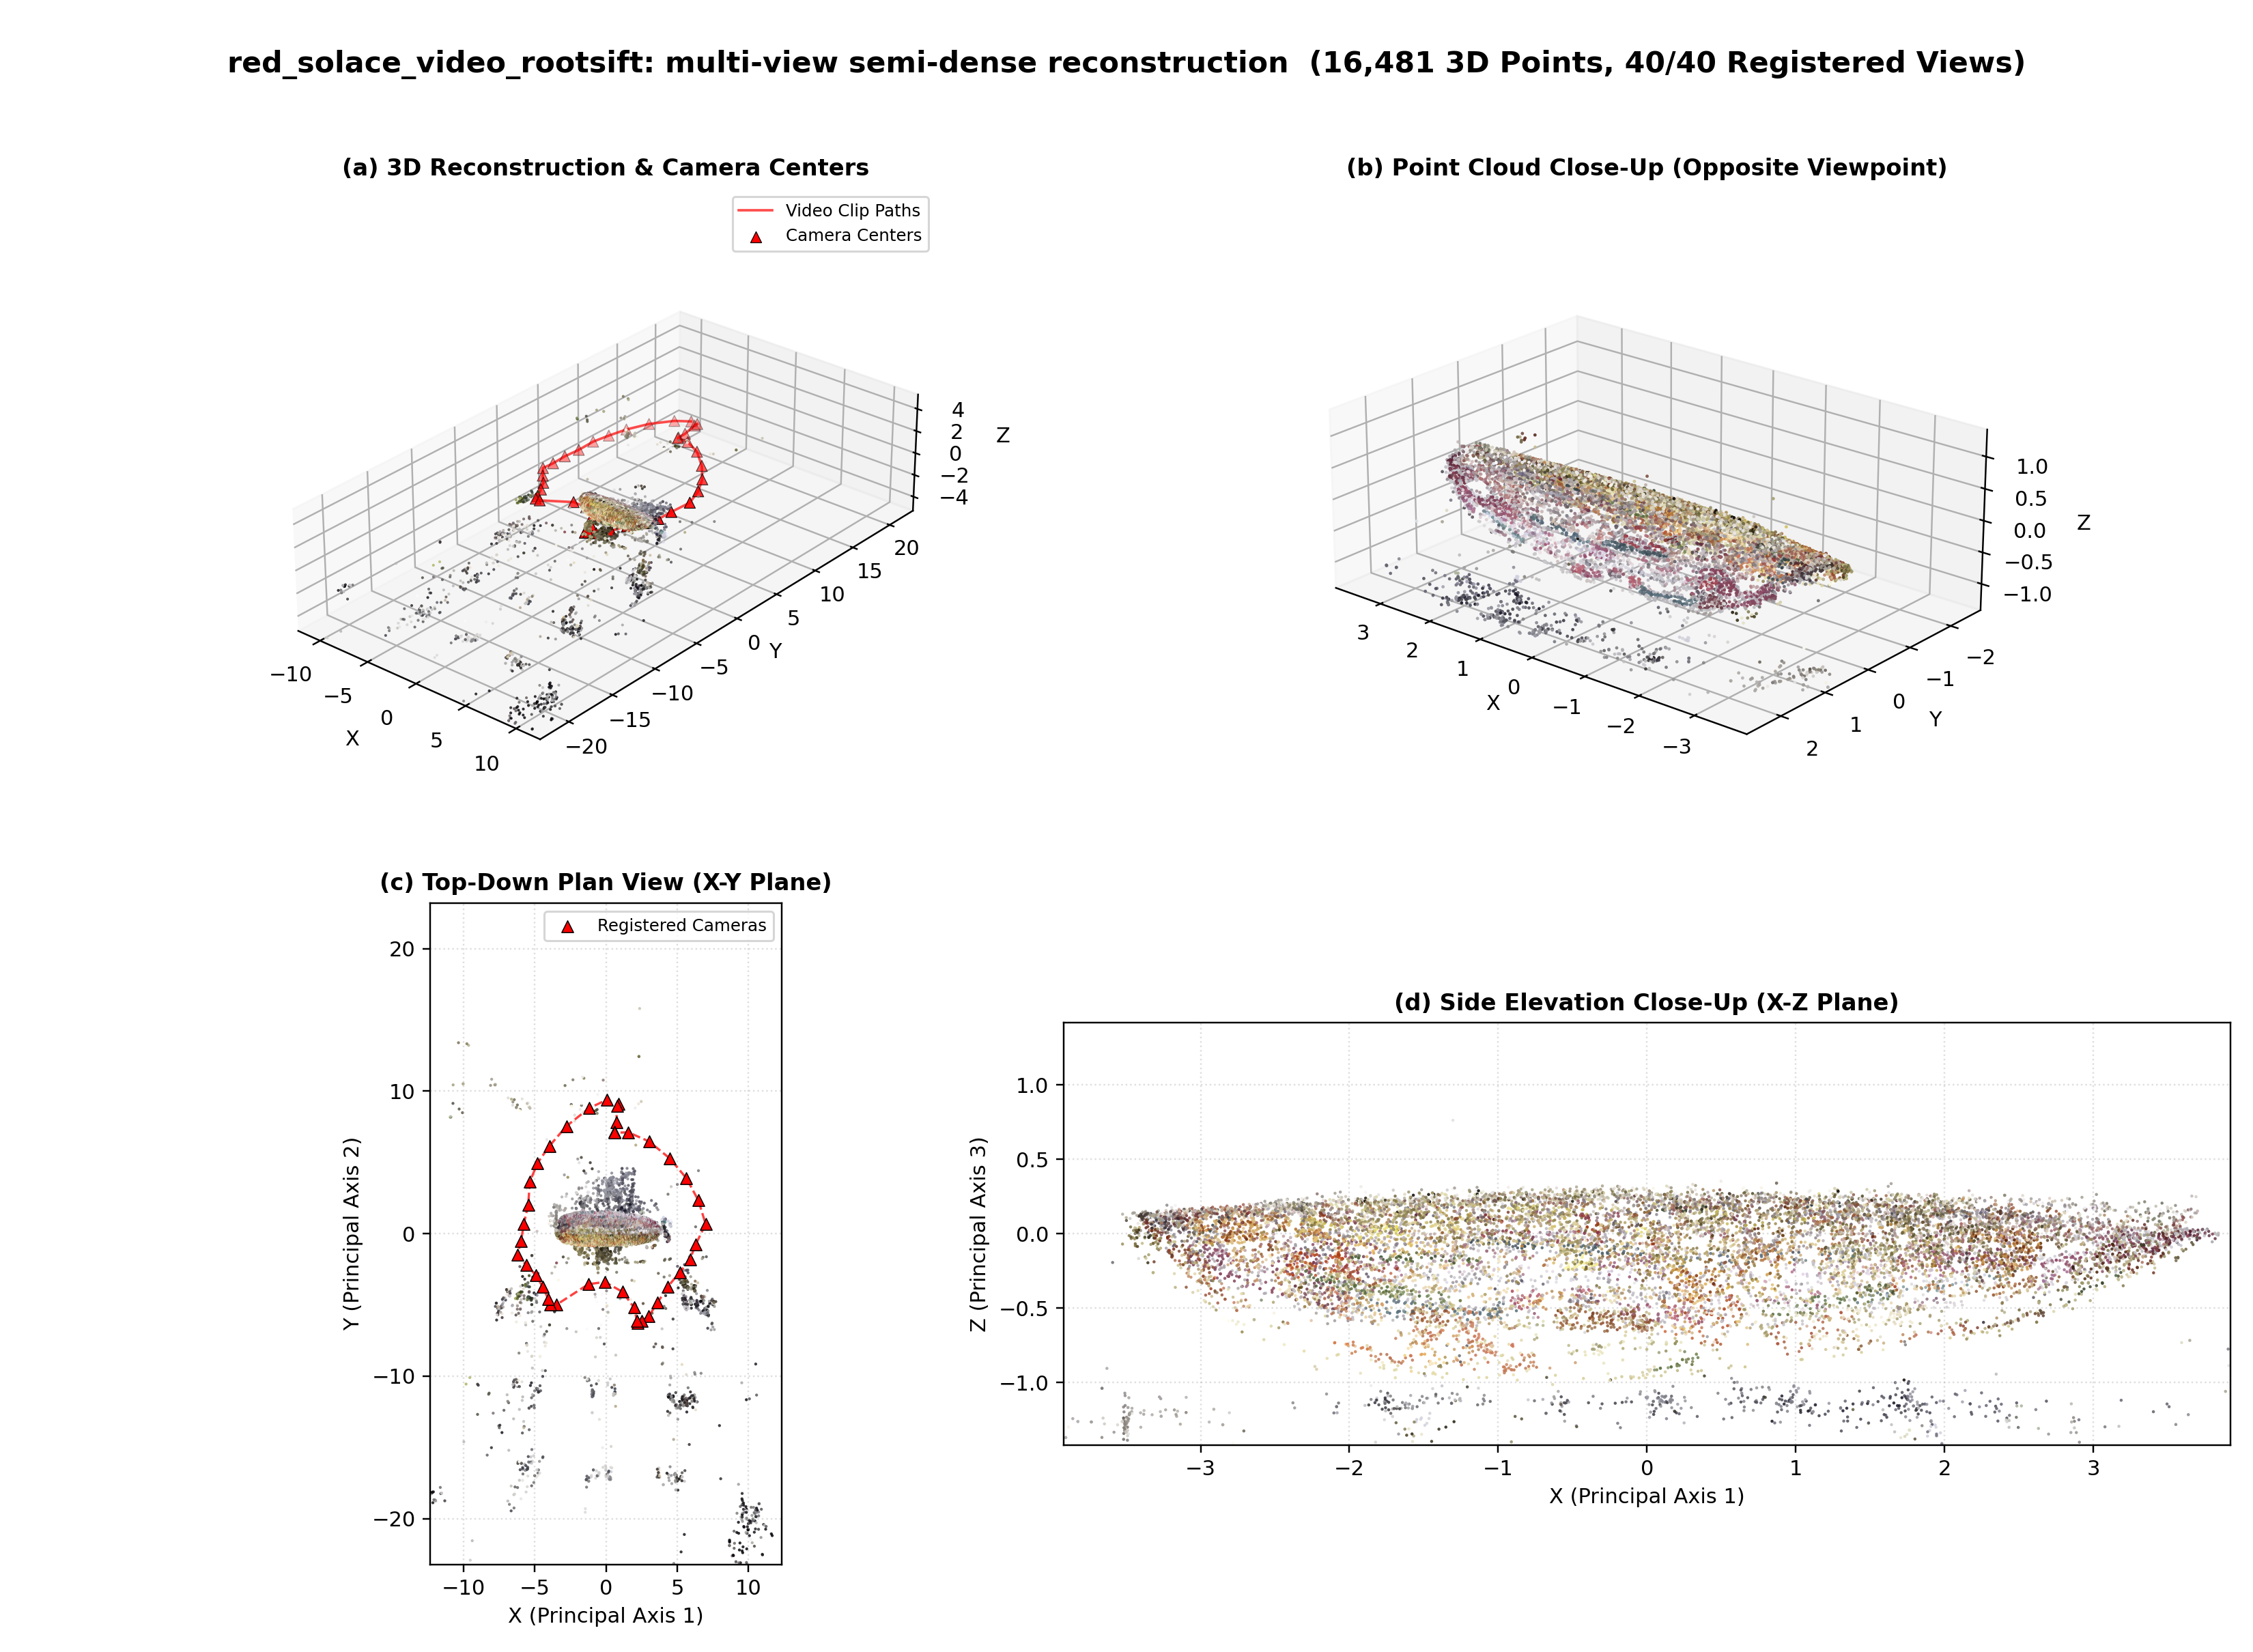
\includegraphics[width=0.96\linewidth]{red_solace_video_rootsift_semi_dense_3d.png}
\captionof{figure}{Red Solace 003, revised semi-dense output. The side and
top views show the boat outline. Background points and uneven support
remain visible. The count includes the sparse landmarks.}
\end{minipage}

\vspace{0.35cm}
\begin{minipage}{\linewidth}
\centering
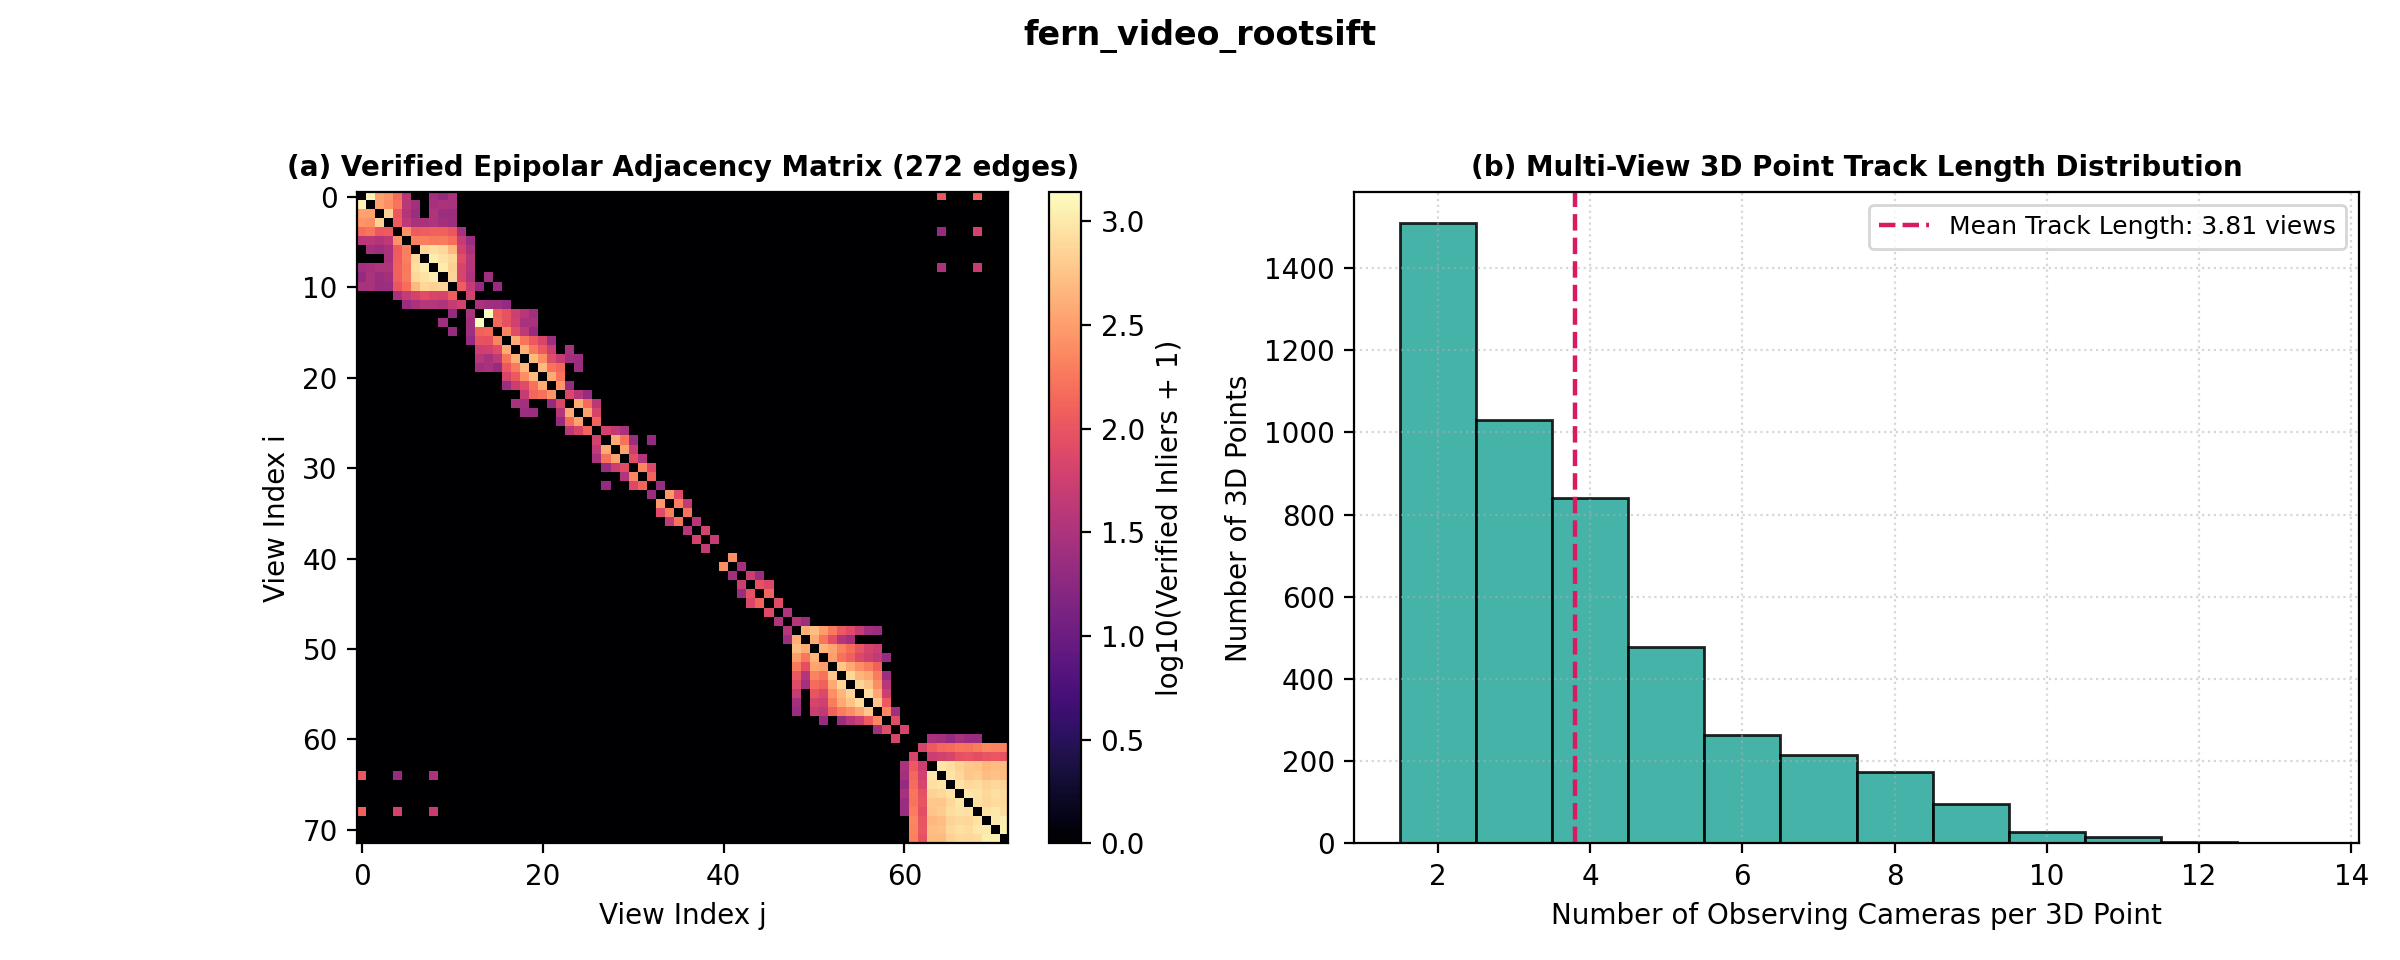
\includegraphics[width=0.96\linewidth]{fern_video_rootsift_scene_graph.png}
\captionof{figure}{Fern 006, verified image-pair graph and landmark track
lengths. The largest match component contains all 72 input frames. Only 24
frames could be registered to a single reconstruction.}
\end{minipage}

\clearpage
\subsection{Red Solace camera localization across six videos}
\label{sec:red-multivideo}
We used clip 003's 12,693 sparse landmarks and 40 registered poses as the
reference map. We sampled eight frames at evenly spaced frame indices from
each of the other five clips. From clip 003, we used every second registered
image as an anchor. We projected the saved 3D landmarks into these 20 anchor
images and associated their projections with nearby RootSIFT keypoints.
Matching a new frame to the anchors then linked its 2D keypoints to the
reference map's 3D landmarks.

We estimated each new pose with EPnP and RANSAC \cite{epnp}, testing five
initial focal lengths and refining the pose and focal length jointly with a
robust reprojection loss. An accepted pose required positive-depth inliers
within four pixels, sufficient image coverage and support from at least two
anchors. The 33 accepted new poses each had at least 55 inliers and a median
inlier reprojection error below 2.48 pixels at the working resolution. The
new frames were localized against the fixed map, so their poses share clip
003's coordinate system and relative scale. The cloud in
Figure~\ref{fig:red-multivideo} is the reference reconstruction.

\begin{center}
\small
\begin{tabular}{@{}lrrrrrrr@{}}
\toprule
\textbf{Clip} & \textbf{001} & \textbf{002} & \textbf{003} & \textbf{004} &
\textbf{005} & \textbf{006} & \textbf{Total}\\
\midrule
Frames evaluated & 8 & 8 & 40 & 8 & 8 & 8 & 80\\
Poses registered & 8 & 8 & 40 & 5 & 4 & 8 & 73\\
\bottomrule
\end{tabular}
\end{center}

\begin{minipage}{\linewidth}
\centering
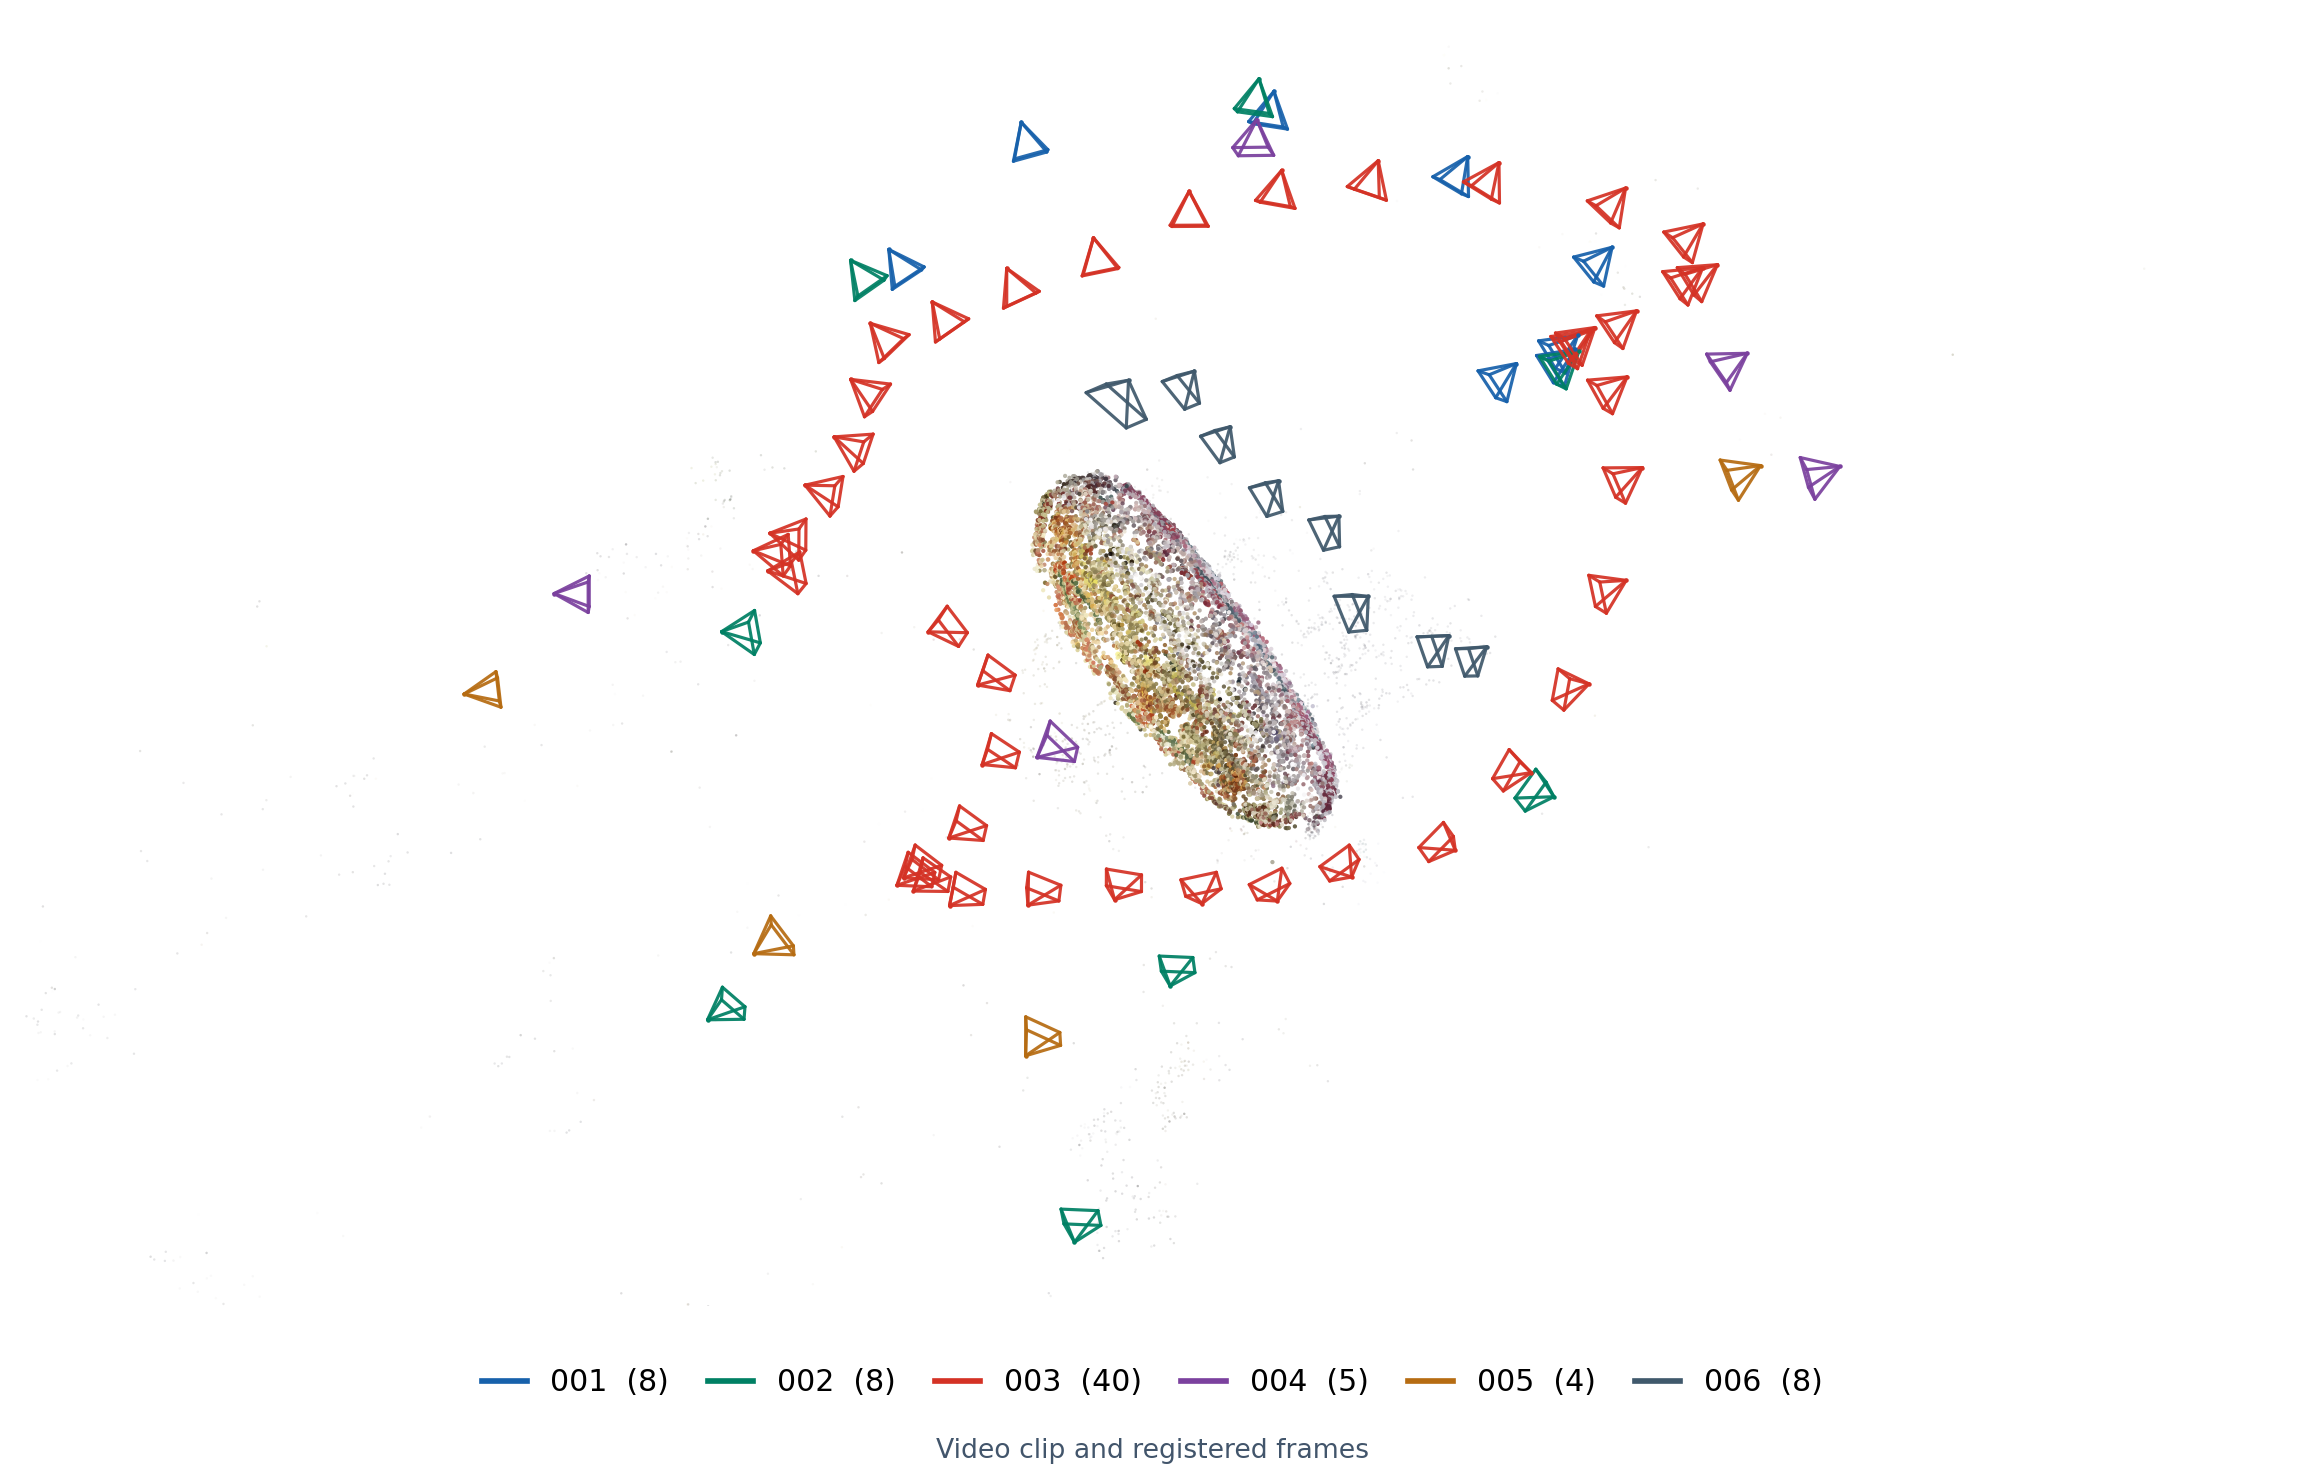
\includegraphics[width=0.88\linewidth]{red-solace-multi-video-cameras.png}
\captionof{figure}{Red Solace sparse reference cloud with 73 registered
camera poses. Each colored frustum shows an estimated camera position and
orientation. The legend gives the number of accepted poses per clip.}
\label{fig:red-multivideo}
\end{minipage}

\clearpage
\section{Stereo surface reconstruction and visualization}
\label{sec:surface}
\subsection{Estimating and validating depth}
We use the registered SfM cameras to rectify overlapping image pairs and
estimate disparity with OpenCV's semi-global block matching
\cite{hirschmuller}. The sparse points constrain the disparity search.
We reject pixels with inconsistent left-to-right and right-to-left disparity
or poor photometric agreement. Accepted disparities are back-projected into the
SfM coordinate frame and checked against another stereo depth estimate. This
cross-view check follows the principle of geometric consistency in multi-view
stereo \cite{mvs}. Foreground silhouettes and scene bounds restrict surface
construction to the sculpture.

\subsection{Red Solace}
The Red Solace 003 run produced 1,251,248 stereo samples after the consistency
checks. A region crop, ground rejection and nine annotated silhouettes retained
921,438 samples from 35 reference depth maps. We fused these observations in
a truncated signed-distance field (TSDF) \cite{curless}. For a voxel at
\(X\), a depth map contributes \(D_i(u_i(X))-z_i(X)\) near the measured
surface, where \(u_i\) and \(z_i\) give its projected pixel and camera depth.
We combine consistent contributions from at least two reference views on a
grid with 0.030-unit spacing in the SfM coordinate system.

Marching cubes extracts the zero level set. We retain crossings supported by
observed grid values and close to depth samples. The exported surface has
34,144 vertices and 63,770 triangles. Its largest connected component
contains 99.1\% of the triangles. The long opening remains visible. Gaps near
its rim and along the underside mark areas with limited observations.

\vspace{0.25cm}
\begin{minipage}{\linewidth}
\centering
\surfacecomparison{red_solace_surface_views.png}
\captionof{figure}{Red Solace surface from clip 003. All three panels use
the same 63,770 triangles and viewpoint. The wireframe shows connectivity,
and the normal colors show the change in surface orientation around the
hull and the upper rim.}
\label{fig:redmesh}
\end{minipage}

\clearpage
\subsection{Fern}
The Fern 006 run in Section~\ref{sec:evaluation} leaves a gap between its registered opening
and closing frames. For the surface experiment we used a separate set of
poses from the archived 002 and 004 clips, which observe the ribs from a
wider range of directions. Stereo produced 77,696 consistent depth samples
across 17 reference views. The most coherent surface came from frame 662 of
clip 004, paired with frame 588. The final mesh uses this reference view's
depth samples after cross-view checks and foreground filtering.

We triangulated the accepted samples in the reference image with a 2D
Delaunay triangulation and used their recovered 3D coordinates for the
mesh. Edges longer than 7.5 pixels or beyond a depth-dependent 3D limit were
discarded. Removing small disconnected patches suppressed isolated fragments.
The resulting mesh has 13,050 vertices and 22,557 triangles. It recovers
parts of the visible wooden ribs and base. The gaps between recovered patches
and the unseen reverse side remain open.

\vspace{0.25cm}
\begin{minipage}{\linewidth}
\centering
\surfacecomparison{fern_surface_views.png}
\captionof{figure}{Fern's observed surface from frame 662 of clip 004.
The colored rendering shows the recovered wooden ribs, the wireframe
reveals discontinuities, and the face-normal colors show orientation
changes along the curved wood.}
\label{fig:fernmesh}
\end{minipage}

\subsection{Rendering and export}
The colored view uses image-derived vertex colors. The wireframe draws the
same mesh edges. For a triangle with vertices \(p_0,p_1,p_2\), the unit face
normal is the normalized cross product
\((p_1-p_0)\times(p_2-p_0)\). In the normal view its components in the
display frame are mapped to RGB by \((n+1)/2\). Both objects are provided
as colored GLB meshes and as PLY meshes with vertex normals. The surfaces
are expressed in relative SfM scale, and the observed gaps are visible
in all three renderings.

\clearpage
\section{Ablations and limitations}
\subsection{Descriptor comparison}
RootSIFT, SIFT and ORB use the same 40 Red Solace frames, feature budget,
ratio threshold and geometry settings. Each descriptor uses its appropriate
distance. This comparison uses a shared configuration for all three methods.

\begin{center}
\small
\begin{tabularx}{\linewidth}{@{}Yrrrr@{}}
\toprule
\textbf{Descriptor} & \textbf{Registered} & \textbf{Sparse points} &
\textbf{Median (px)} & \textbf{P90 (px)}\\
\midrule
RootSIFT & 40/40 & 12,693 & 0.498 & 1.527\\
SIFT     & 40/40 & 12,374 & 0.545 & 1.654\\
ORB      & 18/40 & 4,250  & 0.703 & 1.804\\
\bottomrule
\end{tabularx}
\end{center}

RootSIFT and SIFT have equal registration coverage on this clip. ORB
registers fewer frames under the chosen settings. Residuals describe each
method's retained observations. The RootSIFT final bundle-adjustment pass
reduces the mean residual from 0.796 to 0.760 pixels on observations of the
same 1,800 active landmarks, a subset of the full sparse reconstruction.

\subsection{Sensitivity to the initial focal factor}
The 72 selected Fern frames and their 716 raw matched image pairs were held
fixed while varying the focal prior. Shared focal refinement was enabled
in all four runs.

\begin{center}
\small
\begin{tabularx}{\linewidth}{@{}Yrrrr@{}}
\toprule
\textbf{Initial factor} & \textbf{Registered} & \textbf{Sparse points} &
\textbf{Median (px)} & \textbf{P90 (px)}\\
\midrule
0.72 & 24/72 & 4,833 & 0.685 & 1.889\\
0.85 & 24/72 & 3,748 & 0.910 & 2.436\\
0.95 & 24/72 & 4,657 & 0.761 & 1.962\\
1.05 & 24/72 & 4,100 & 0.705 & 2.134\\
\bottomrule
\end{tabularx}
\end{center}

The focal factors change residuals and point counts while leaving registration
at 24 frames. A connected graph records verified two-view matches.
Incremental registration additionally needs enough of a new frame's observations
to correspond to the current 3D landmarks. Repeated wood texture, changes in
object scale, and gaps in stable tracks are plausible contributors to Fern's
missing interval. Measured calibration and overlapping bridge views would
help separate these effects in a further test.

\section{Conclusion}
The revised mapper increases Fern registration on a fixed archived input.
Red Solace supports multi-view depth fusion and a largely connected hull
surface. Fern's narrower reliable coverage supports an observed mesh patch
from the archive, with gaps between the reconstructed ribs. The registration
and reprojection statistics measure coverage and fit to image observations.
Absolute scale, independent surface error and loop-closure error remain
unevaluated.

\clearpage
\section*{Reproducibility}
The implementation uses OpenCV for feature detection, two-view estimation and
PnP, and SciPy for sparse nonlinear least squares. The project source
implements incremental mapping, track construction and feature-based fusion.
Run the commands from the project root.

\begin{verbatim}
python -m pip install -r requirements.txt
python run_experiments.py
python -m tools.red_solace_surface
python -m tools.fern_surface_patch
\end{verbatim}
The surface commands use the bundled keyframes, pose records and depth
samples. The Fern replay inputs are in \path{outputs/validation/fern_archive/},
and the command writes to its \path{reproduced/} folder. The delivered meshes
are under \path{outputs/final/}. The six-video pose file and overlay are in
\path{outputs/case-study/}. See the README for the stereo, camera
localization and rendering commands.

\begin{center}
\small
\begin{tabularx}{\linewidth}{@{}lY@{}}
\toprule
\textbf{Source} & \textbf{Role}\\
\midrule
\code{sfm/data.py}, \code{sfm/features.py} & Keyframes, calibration, descriptors and matches\\
\code{sfm/geometry.py}, \code{sfm/tracks.py} & Pair verification and consistent feature tracks\\
\code{sfm/pipeline.py}, \code{sfm/bundle_adjustment.py} & Registration, triangulation and refinement\\
\code{sfm/densify.py}, \code{sfm/visualization.py} & Multi-view feature fusion and export\\
\code{run_experiments.py} & Inputs, settings, ablations and result generation\\
\code{tools/} & Stereo depth, surface extraction and three-panel rendering\\
\bottomrule
\end{tabularx}
\end{center}

\begin{thebibliography}{9}
\small
\setlength{\itemsep}{3pt}
\setlength{\parsep}{0pt}
\bibitem{hartley} R. Hartley and A. Zisserman, \emph{Multiple View Geometry in
Computer Vision}, 2nd ed. Cambridge University Press, 2003.
\bibitem{schonberger} J. L. Sch{\"o}nberger and J.-M. Frahm, Structure-from-motion
revisited, \emph{CVPR}, pp. 4104--4113, 2016.
\bibitem{rootsift} R. Arandjelovi{\'c} and A. Zisserman, Three things everyone
should know to improve object retrieval, \emph{CVPR}, pp. 2911--2918, 2012.
\bibitem{epnp} V. Lepetit, F. Moreno-Noguer, and P. Fua, EPnP: An accurate
\(O(n)\) solution to the PnP problem, \emph{IJCV}, vol. 81, pp. 155--166, 2009.
\bibitem{triggs} B. Triggs, P. McLauchlan, R. Hartley, and A. Fitzgibbon,
Bundle adjustment---a modern synthesis, \emph{Vision Algorithms:
Theory and Practice}, pp. 298--372, 2000.
\bibitem{mvs} J. L. Sch{\"o}nberger, E. Zheng, J.-M. Frahm, and M. Pollefeys,
Pixelwise view selection for unstructured multi-view stereo,
\emph{ECCV}, pp. 501--518, 2016.
\bibitem{hirschmuller} H. Hirschm{\"u}ller, Stereo processing by semiglobal
matching and mutual information, \emph{IEEE TPAMI}, vol. 30, no. 2,
pp. 328--341, 2008.
\bibitem{curless} B. Curless and M. Levoy, A volumetric method for building
complex models from range images, \emph{SIGGRAPH}, pp. 303--312, 1996.
\end{thebibliography}
\end{document}
